%% \begin{itemize}
%% \item[{\bf Week of June 8}] Peeragogy Project and Roadmap, comments \#17--\#27.  JC: I've made an initial revision, changing ``Peeragogy Project'' to ``Peeragogy''.  See text in green below.  Roadmap is orange, meaning ``on deck'' but no major changes have been made there yet.
%% \item[{\bf Week of June 15}] Use or Make and Carrying Capacity, comments up to \#36.  JC: I've made initial revisions, circulated by email.  Lisa has given some thoughtful comments there, some of that has been merged in here but not all. ``Use or Make'' now retitled as ``Reduce, Reuse, Recycle''.
%% \item[{\bf Week of June 22}] A Specific Project and Wrapper.  JC: I've revised ``A Specific Project''.  I'm wondering if some of the other items in our upcoming list are redundant.  Specifically, I think ``Creating a Guide'' could be combined with ``Roadmap'' and ``Scrapbook'' could be combined with ``Pattern Audit Routine''.  This would save us a week of time and perhaps we could use that to get some more feedback.  It would also save some space in the final paper.
%% \item[{\bf Week of June 29}] Heartbeat and Creating a Guide
%% \item[{\bf Week of July 6}] Newcomer and Pattern Audit Routine
%% \item[{\bf Week of July 13}] Scrapbook and Distributed Roadmap
%% \item[{\bf Week of July 20}] Make sure to submit the revised paper
%% \end{itemize}

\section{Introduction}\label{sec:Introduction}

Readers will have encountered \emph{peer production}, at least in applications like Wikipedia, StackExchange, and free/libre/open source software development.   In the Peeragogy project,  we aim to build upon these inspiring examples to help design the future of education.  
We have found design patterns tremendously useful for organizing our thinking about these matters.  However, there is a key difference between our pattern catalog and previous collections of design patterns that touch on similar domains -- like \emph{Liberating Voices: A Pattern Language for Communication Revolution} \cite{schuler2008liberating} and \emph{Pedagogical Patterns: Advice for Educators} \cite{bergin2012pedagogical}.  Our pattern catalog is our primary project management tool -- our way of ``synthesizing form'' \cite{alexander1964notes}.

A convincing implementation of Christopher Alexander’s idea of patterns as a ``living language'' \cite[p.~xvii]{alexander1977pattern} was realized with one of the earliest applications of wiki software developed by Ward Cunningham: the Portland Pattern Repository.  What we have developed is a further iteration of this idea.   As our patterns developed, the pattern template we used was revised and revised again, until ultimately we settled on something quite traditional.  At the level of the template, our one innovation is to add a ``What's next'' annotation to each pattern, which anticipates the way the pattern will continue to ``resolve'' in the context of our project. 

% The patterns we introduce here focus on negotiating the execution and implementation of solutions in their practical context.
%  This often requires compromise, adjustments and even restarts.  

At a more philosophical level, our approach is all about human interaction, and the challenges, fluidity and lack of predictability that comes with it.  Something that works for one person may not work for another or may not even work for the same person in a slightly different situation.  It is easy to say ``just do X'' and even somewhat easy for reasonable people to agree in general terms about what to do.  In our view, other pattern languages often achieve this sort of common sense rationality, and then stop.  In our experience, failure in the prescriptive model begins when people start trying to define things more carefully and make context-specific changes -- when they actually try to put ideas into practice.  One is put in mind of Alfred Korzybski's famous remark: ``the map is not the territory.''  

Our aim in this paper is to outline a new approach to education drawing on the principles of free/open/libre software and ``open culture.''  In order to do this, we attempt to discuss these principles in an actionable, hands-on way.  Mako Hill suggests that one recipe for success in peer production projects is to take a familiar idea -- the canonical example is an \emph{encyclopedia} -- and make it easy for people to participate in building it \cite{almost-wikipedia}.  Here, our inspiring familiar idea is the \emph{university}.  If this is the map (Figure \ref{madison-map}), then the territory is the tacitly-familiar idea of peeragogy.  

\begin{wrapfigure}{l}{.52\textwidth}
\vspace{-.3cm}
\begin{center}
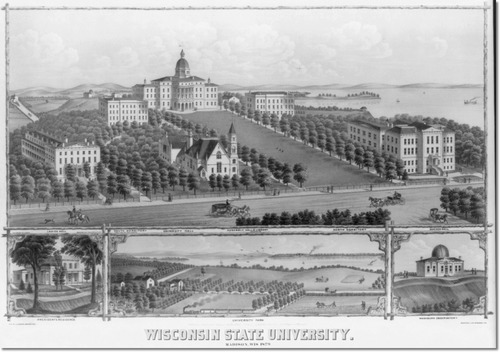
\includegraphics[width=.5\textwidth,trim=0 30 10 2, clip=true]{wisconsin-map}
\end{center}
\vspace{-.1cm}
\caption{A prototypical university.  Caption reads: ``Wisconsin State
  University, Madison, Wis. 1879''.  Inset captions describe the
  pictured buildings: ``Ladies Hall, South Dormitory, University Hall,
  Assembly Halls \& Library, North Dormitory, Science Hall, President's
  Residence, University Farm, and Washburn Observatory.''  Public
  domain.\label{madison-map}}
\vspace{-.3cm}
\end{wrapfigure}

The model university is not separate from the life of the state or its
citizenry, but aims to ``assume leadership in the application of
knowledge for the direct improvement of the life of the people in
every sphere'' \cite[p. 88]{curti1949university}.  We have framed our
considerations here in terms of the future of ``education,'' however,
peeragogy is not just for teachers and students, but for anyone with a
commitment to learning.  We use the patterns of peeragogy to
\emph{constitute and occupy practical or speculative problems as such}
\cite[p.~204]{deleuze1994difference}.
%
Our patterns are a living language just insofar as they are hooked to
action.

% Till Sch{\"u}mmer \emph{et al.}~have emphasized that pattern authors ``talk about what by definition is tacit'' and highlight the role of nonverbal communication ``needed to communicate the unspeakable'' \cite[p.~9]{schummer2014beyond}.

The essence of peeragogy is to combine an accessible approach with reflective practice.   We seek to develop a richer understanding of collaborative interaction.  This work is relevant to giving the often vague idea of ``openness'' a more concrete meaning, and will have applications within and beyond peer production.  Our approach to emergent organization is likely to be of interest to theorists in fields like organization studies and, perhaps surprisingly, computer science, where researchers are increasingly making use of social approaches to software design and development (e.g., via the \href{http://www.agilemanifesto.org/}{Manifesto for Agile Software Development}) as well as agent-based models of computation and learning \cite{minsky1967programming,poetry-workshop}.

The next section introduces \patternname{Peeragogy} more explicitly in the form of a design pattern, and Sections \ref{sec:Roadmap}--\ref{sec:Scrapbook} describe the other patterns in our catalog.  Figure \ref{fig:connections} illustrates their interconnections.  The key forces that apply within the context of these patterns are highlighted in bold face.  Section \ref{sec:Distributed_Roadmap} collects our ``What's next'' steps and summarizes the outlook of our project. Section \ref{sec:Conclusion} reviews the contributions made in the paper, positioning this work as a hands-on complement to existing sociological and historical research on peer production (surveyed in \cite{benkler2015peer}).

\begin{figure}
\vspace{-.9in}
{\centering
\begin{tikzpicture}[dot/.style={circle,inner sep=1pt,fill,name=#1}]
%\draw[step=1cm,gray,very thin] (0,0) grid (10,10);
\node (assess) at (5, 9.75) {{\Large {\sc Assess}}};
\node (organize) at (5, 0) {{\Large {\sc Organize}}};
\node (cooperate)[text width=2cm,align=center,rotate=270] at (10, 5) {{\Large {\sc Convene}}};
\node (convene)[text width=15cm,align=center,rotate=90] at (0, 5) {{\Large {\sc Cooperate}}};

\node(legend)[draw,rectangle,text width=2.67cm] at (9.25,.75) 
{\begin{tabular}{p{2.7cm}@{\hspace{-1mm}}}
\textbf{Legend}\\ \hline\vspace{-2mm} \textbf{A}\hspace{.41in}\textbf{B}\\
if pattern \textbf{A} refers to pattern \textbf{B}.
  \end{tabular}};
\draw[-{Latex[width=2mm]},draw=gray] ([xshift=5mm,yshift=1.75mm]legend.west) -- ([xshift=-14.8mm,yshift=1.75mm]legend.east);

%%%%%%%%%%%%%%%%%%%%%%%%%%%%%%%%%%%%%%%%%%%%%%%%%%%%%%%%%%%%%%%%%%%%%%%%%%%%%%%%%%%%%%%%%%%%%%%%%%%%%
\node[below = 5cm of assess] (roadmap) {\ref{sec:Roadmap}. \hyperref[sec:Roadmap]{\emph{Roadmap}}};
\node (reduce) at (5, 8.75) {\ref{sec:Reduce, reuse, recycle}. \hyperref[sec:Reduce, reuse, recycle]{\emph{Reduce, reuse, recycle}}};
\node (carryingcapacity) at (1.25, 7.15) {\ref{sec:Carrying capacity}. \hyperref[sec:Carrying capacity]{\emph{Carrying capacity}}};
\node[below = 3.2cm of carryingcapacity] (heartbeat) {\ref{sec:Heartbeat}. \hyperref[sec:Heartbeat]{\emph{Heartbeat}}};
\node (aspecificproject) at (8.5, 6.5) {\ref{sec:A specific project}. \hyperref[sec:A specific project]{\emph{A specific project}}};
\node[below = 1cm of roadmap] (wrapper) {\ref{sec:Wrapper}. \hyperref[sec:Wrapper]{\emph{Wrapper}}};
\node (newcomer) at (8.5, 3.25) {\ref{sec:Newcomer}. \hyperref[sec:Newcomer]{\emph{Newcomer}}};
\node[below = 1.7cm of wrapper] (scrapbook) {\ref{sec:Scrapbook}. \hyperref[sec:Scrapbook]{\emph{Scrapbook}}};
\node[above = 1cm of aspecificproject] (peeragogyproject) {\ref{sec:Peeragogy}. \hyperref[sec:Peeragogy]{\emph{Peeragogy}}};
%%%%%%%%%%%%%%%%%%%%%%%%%%%%%%%%%%%%%%%%%%%%%%%%%%%%%%%%%%%%%%%%%%%%%%%%%%%%%%%%%%%%%%%%%%%%%%%%%%%%%
\draw[-{Latex[width=2mm]},draw=gray] (peeragogyproject) -- (aspecificproject);
% \draw[-{Latex[width=2mm]},draw=gray] (aspecificproject) -- (par);
\draw[-{Latex[width=2mm]},draw=gray] (aspecificproject) -- (roadmap);
\draw[-{Latex[width=2mm]},draw=gray] (aspecificproject.230) to[out=250,in=40] (scrapbook);
\draw[-{Latex[width=2mm]},draw=gray] (aspecificproject) -- (carryingcapacity);
\draw[-{Latex[width=2mm]},draw=gray] (carryingcapacity.337) -- (newcomer);
\draw[-{Latex[width=2mm]},draw=gray] (carryingcapacity.330) -- (roadmap);
\draw[-{Latex[width=2mm]},draw=gray] (carryingcapacity) -- (peeragogyproject);
\draw[-{Latex[width=2mm]},draw=gray] ([xshift=1mm]carryingcapacity.south) -- (scrapbook.140);
% \draw[-{Latex[width=2mm]},draw=gray] ([xshift=2mm]creatingaguide.160) to[out=-215,in=-67] (carryingcapacity);
\draw[-{Latex[width=2mm]},draw=gray] (heartbeat) -- (aspecificproject.185);
\draw[-{Latex[width=2mm]},draw=gray] (heartbeat) -- (carryingcapacity);
\draw[-{Latex[width=2mm]},draw=gray] (heartbeat) -- (scrapbook.155);
\draw[-{Latex[width=2mm]},draw=gray] (heartbeat) -- (reduce.215);
\draw[-{Latex[width=2mm]},draw=gray] (newcomer) -- ([xshift=4mm]reduce.south);
\draw[-{Latex[width=2mm]},draw=gray] (newcomer) -- (aspecificproject);
% \draw[-{Latex[width=2mm]},draw=gray] (newcomer) -- (creatingaguide.north);
\draw[-{Latex[width=2mm]},draw=gray] (newcomer) -- (roadmap.350);
\draw[-{Latex[width=2mm]},draw=gray] (newcomer) -- (scrapbook.24);
% \draw[-{Latex[width=2mm]},draw=gray] (par) -- (scrapbook);
\draw[-{Latex[width=2mm]},draw=gray] (roadmap) -- (peeragogyproject.195);
\draw[-{Latex[width=2mm]},draw=gray] (roadmap.350) -- (newcomer);
\draw[-{Latex[width=2mm]},draw=gray] (roadmap) -- (wrapper);
\draw[-{Latex[width=2mm]},draw=gray] ([yshift=.3mm]roadmap.west) -- (heartbeat);
\draw[-{Latex[width=2mm]},draw=gray] (roadmap) -- (aspecificproject);
% \draw[-{Latex[width=2mm]},draw=gray] (scrapbook) -- (par);
\draw[-{Latex[width=2mm]},draw=gray] (scrapbook) -- (wrapper);
\draw[-{Latex[width=2mm]},draw=gray] (scrapbook.110) to[out=123,in=250] (reduce.245);
\draw[-{Latex[width=2mm]},draw=gray] (scrapbook.70) to[out=43,in=305] (roadmap.330);
% \draw[-{Latex[width=2mm]},draw=gray] ([xshift=2mm,yshift=-.4mm]reduce.south) -- (creatingaguide);
\draw[-{Latex[width=2mm]},draw=gray] (reduce) -- (carryingcapacity);
\draw[-{Latex[width=2mm]},draw=gray] (reduce) -- (roadmap);
\draw[-{Latex[width=2mm]},draw=gray] ([xshift=.7mm]wrapper.175) -- (heartbeat);
\draw[-{Latex[width=2mm]},draw=gray] ([xshift=-.7mm,yshift=-.3mm]wrapper.360) -- (newcomer);
\draw[-{Latex[width=2mm]},draw=gray] (wrapper) -- ([xshift=2.3mm]carryingcapacity.south);
\draw[-{Latex[width=2mm]},draw=gray] (wrapper) -- (roadmap);

\end{tikzpicture}


\par
}
\vspace{-.9in}
\caption{Connections between the patterns of peeragogy.  An arrow points from pattern \textbf{A} to pattern \textbf{B} if the description of pattern \textbf{A} references pattern \textbf{B}. Labels at the borders of the figure correspond to the main sections of the \emph{Peeragogy Handbook}.\label{fig:connections}}
\end{figure}

% deferring a more detailed elaboration of next steps in the educational arena to future work that will build on this basis.
% Technology has come a long way since Alexander suggested ``you will get the most `power' over the language, and make it your own most effectively, if you write the changes in, at the appropriate places in the book'' \cite[p.~xl]{alexander1977pattern}.
% While Christian Kohls insightfully describes patterns as the unique resolution of the dynamical forces acting in a given context \cite{kohls2010structure,kohls2011structure}.
%%% Patterns come to you through mindful awareness ... Charlotte: I think about patterns all the time now, I think about what makes me productive in a team.
% So, while we speak the same language as other developers of design patterns, our orientation is somewhat different, and our understanding of the word `pattern' is nuanced because we aim to take full account of the lifecycle of patterns.  Our work contributes to a recent ``performative'' turn \cite{schummer2014beyond}, which we believe gets at the heart of what design patterns can do.
%  
% In practical terms, we believe the patterns that we introduce here will be useful for students and educators who want their work to have real-world relevance, to activists and policy-makers who want to develop practicable solutions to large-scale problems, and to employees and managers who, like it or not, find themselves working in distributed teams. 
